\documentclass[10pt,a4paper]{amsart}
\usepackage{macros}

\begin{document}
\bibliographystyle{alpha}

\noindent \textit{Algebraic Number Theory, Math 421}

\noindent \textit{Instructor: Sreekar M. Shastry}

\noindent \emph{Notes on the splitting of primes in extensions and quadratic reciprocity}

\section{Ramification}

\begin{terminology}
A number ring is the ring of integers in a number field.
\end{terminology}

Let us mention the following theorem, purely for curiosity.

\begin{thm}
Let $\O$ be a number ring and let $\alpha\in \O$ be of degree $n$ over \Q{}.
Then there is an integral basis \[\left\{ 1,\frac{f_1(\alpha)}{d_1}, \dots,
\frac{f_{n-1}(\alpha)}{d_{n-1}} \right\}\] where $d_i\in \Z$ satisfy
$d_1|d_2|\cdots|d_{n-1}$, the $f_i\in \Z[x]$ are monic, and $\deg f_i = i.$ The
$d_i$ are uniquely determined. See \cite[13, p.36]{M}.
\end{thm}

\begin{terminology}
What is called ``inertial degree'' on \cite[p.64]{M} is more often called the
``residual degree.''
\end{terminology}

\begin{defn}
Let $L/K$ be an extension of number fields. A prime $P$ of $\O_K$ is said to be
ramified in $\O_L$ if $e(Q/P) > 1$ for some prime $Q$ of $K$ lying above it, or
equivalently, if $P.\O_L$ is not squarefree.
\end{defn}

Let us recall the following theorem \cite[21, p.65]{M} and a generalization.

\begin{thm}
Let $L/K$ be a finite extension of number fields and let $Q_1,\dots,Q_g$ be the
primes of $\O_L$ lying above a prime $P$ of $\O_K.$ Denote by $e_1,\dots,e_r$
and $f_1,\dots,f_r$ the corresponding ramification indices and residual
degrees. Then we have \[ [L:K] = \sum_{i=1}^{g} e_i f_i.\]
\end{thm}

\begin{thm}
Moreover, if $L/K$ is Galois then the $e_i$ and $f_i$ are independent of $i$
and we have \[ [L:K] = efg\] where $g$ is as above and $e$,$f$ is the common
value of the $e_i$,$f_i$, respectively. See \cite[20, p.117]{FT}.
\end{thm}

We recall the following result \cite[23, p.70]{M} which was proved in the
lecture of 7-Feb-11.

\begin{thm}
Let $L/K$ be a normal extension of number fields with Galois group $G$. Then
$G$ acts transitively on the set of primes of $L$ lying above a given prime of
$K$.
\end{thm}

\begin{notation}
For an ideal $I$ of a Dedekind ring $\O$, write \[\norm{I} := \# \O/I.\]
\end{notation}

We have the following important theorem which we will prove a special
case of below.

\begin{rem}
Passages of the notes bounded by \{begin $*$\} and \{end $*$\} are optional and
will not be covered on the exams or homework assignments.
\end{rem}

\noindent \{begin $*$\}

Let $L/K$ be a finite extension of number fields. Then there is a notion of
relative discriminant $$D_{L/K} \in \Cl{\O_K}^2$$ which is to say, $D_{L/K}$ is
a square in the ideal class group of $K$. We will (perhaps?) see the definition
of relative discriminant later on in the course.

Next, let $\O_L^\vee$ be the dual of $\O_L$ with respect to the trace
$\tr_{L/K}$. The inverse of $\O_L^\vee$ in $\Cl{L}$ is known as the
\textit{different} and denoted by $\mathscr{D}_{L/K}$. It can be shown that
\[\Nm_{L/K}(\mathscr{D}_{L/K}) = D_{L/K},\] i.e.~the norm of the different is
the discriminant.

The results we want to state are the following.

\begin{thm}
A prime $P$ ramifies in the extension $L/K$ iff $P|D_{L/K}$.
\end{thm}

\begin{thm}
Let $L=K(\alpha)$ and suppose that $f(x)$, the minimal polynomial of $\alpha$
over $K$, lies in $\O_K[x].$ Then

(a) $\O_K[\alpha]^{\vee} = f'(\alpha)\O_K[\alpha]$, and

(b) $\mathfrak{d}(\O_K[\alpha]) = \Nm_{L/K}(f'(\alpha))\O_K = \disc{f}\O_K$.
\end{thm}

\begin{rem}
In the statement of the theorem, by $\mathfrak{d}(\O_K[\alpha])$ is meant the
absolute discriminant of the ring extension $\O_K[\alpha]/\Z$, regarded as an
ideal in $\Z$ Note well that this notion discards the sign of the absolute
discriminant $\mathrm{disc}(K) \in \Z$.
\end{rem}

\noindent \{end $*$\}

\begin{lem}
Let $K$ be a number field of degree $n$ over \Q{} and let
$\alpha_1,\dots,\alpha_n \in K.$ Then

(a) $\disc{r\alpha_1,\alpha_2,\dots,\alpha_n} =
r^2\disc{\alpha_1,\dots,\alpha_n}$ for all $r\in\Q$ and

(b) if $\beta$ is a \Q-linear combination of $\alpha_2,\alpha_3,\dots,\alpha_n$
then \[\disc{\alpha_1+\beta,\alpha_2,\dots,\alpha_n} =
\disc{\alpha_1,\dots,\alpha_n}.\]
\end{lem}

\begin{proof}
Expand out the determinant which defines the discriminant. (Recall that the
discriminant of an $n$-tuple $(\alpha_i)_{i=1}^n$ in $\O_K$ is
$|\sigma_i(\alpha_j)|^2$ i.e.~the square of the determinant of the matrix with
the given $ij$th entry, where the $\sigma_i$ are the embeddings of $K$ into
\C.)
\end{proof}

The following statement and proof are from \cite[p. 72ff]{M}.

\begin{thm}
Let $p$ be a prime in \Z{} and suppose that $p$ is ramified in a number ring
$\O_K$. Then $p | \disc{\O_K}.$
\end{thm}

\begin{proof}
Let $P$ be a prime of $\O_K$ lying over $p$ such that $e(P/p) > 1$. Then $p.\O
= P.I$ where $I$ is divisible by all primes of $\O_K$ lying over $p$, including
$P$.

Let $\{\sigma_1,\dots,\sigma_n\}$ be the embeddings of the fraction field $K$
of $\O_K$ into \C{} and extend each $\sigma_i$ to an automorphism of some $L/K$
such that $L$ is normal over \Q{}. Thus the discriminant of an $n$-tuple
$(\alpha_i)_{i=1}^n$ in $\O_K$ is $|\sigma_i(\alpha_j)|^2$ (i.e.~the square of
the determinant of the matrix with the given $ij$th entry).

Let $\{\alpha_1,\dots,\alpha_n\}$ be an integral basis for $\O_K$. We will
replace one of the $\alpha_i$ by a suitably chosen element which will enable us
to see that $p|\disc{\O_K}$. Choose any $\beta \in I\smallsetminus p.\O_K$
(where we know that $p.\O_K \subsetneq I$ --- this is in fact the reason that
$I$ was defined as it was); then $\beta$ is in every prime of $\O_K$ lying over
$p$, but not in $p.\O_K$. Writing \[\beta = m_1\alpha_1 + \cdots + m_n\alpha_n,
m_i\in \Z,\] then the fact that $\beta\notin p.\O_K$ implies that $p\ndiv m_j$
for some $j$. Without loss, suppose that $p\ndiv m_1$. Put \[d := \disc{\O_K} =
\disc{\alpha_1,\dots,\alpha_n};\] then we have by the above lemma
\[\disc{\beta,\alpha_2,\dots,\alpha_n} = m_1^2 d.\] Since $p\ndiv m_1$ it will
suffice to show that \[p | \disc{\beta,\alpha_2,\dots,\alpha_n}.\]

Recall that $\beta$ is in every prime of $\O_K$ lying over $p$. It follows that
$\beta$ is in every prime of $\O_L$ lying over $p$. (Each such prime $Q\ni p$
and $Q\cap \O_K$ is a prime lying over $p$, so that $\beta\in Q\cap\O_K \subset
Q$.) Fixing such a $Q$ of $\O_L$ lying over $p$, we claim that
$\sigma(\beta)\in Q$ for each $\sigma \in \Aut(L/\Q)$. To see this, observe
that $\sigma^{-1}(Q)$ is a prime of $\sigma^{-1}(\O_L)=\O_L$ lying over $p$ and
hence contains $\beta$. Thus $\sigma_i(\beta)\in Q$ for all $i$. It follows by
expanding out the determinant which defines the discriminant that $Q$ contains
$\disc{\beta,\alpha_2,\dots,\alpha_n}$. Since the discriminant is in \Z{}, it
is in $Q\cap \Z = p.\Z$, as required.
\end{proof}

\begin{cor}
Only finitely many primes of \Z{} are ramified in a given number ring $\O_K$.
\end{cor}

\begin{cor}
Let $L/K$ be an extension of number fields. Then only finitely many primes of
$K$ are ramified in $L$.
\end{cor}

%%%%%%%%%%%%%%%%%%%%%%%%%%%%%%%%%%%%%%%%%%%%%%%%%%%%%%%%%%%%%%%%%%%%%%

\section{Inertia and Decomposition}

\begin{defns}
Let $L/K$ be a normal extension of number fields with group $G$ and degree $n =
[L:K]$ with rings of integers \OL,\OK. Let $P$ be a prime of $K$ so that all
primes $Q$ of $L$ lying above it have common ramification index $e$ and
residual degree $f$, and if there are $r$ such primes, we have $efr = n$.

Fix such a $Q$ lying over $P$. The \emph{decomposition group} is \[D(Q/P):=
\{\sigma\in G : \sigma Q = Q\}.\] The \emph{inertia group} is \[I(Q/P) :=
\{\sigma\in G : \sigma(\alpha) \equiv \alpha \imod{Q}, \, \forall \alpha\in
\OL\}.\] These are subgroups of $G$ and we have $I\subset D.$
\end{defns}

For each $\sigma\in G$ we have the commutative diagram \[ \xymatrix{ \OL
\ar[r]^\sigma \ar[d]& \OL\ar[d]\\ \OL/Q \ar[r]^{\overline{\sigma}} & \OL/Q }
\] which gives us the group homomorphism \[D(Q/P) \rightarrow \Gal{k(Q)/k(P)}\]
where we write $k(Q) = \OL/Q$ and $k(P) = \OK/P$ for the resdidue field; these
are finite fields.\footnote{In fact the whole of algebraic number theory can be
developed for a certain class of Dedekind domains such that the residue
fields at maximal ideals are finite fields. Such fields are called ``global
fields'' and consist of number fields which are finite extensions of \Q{} and
the function fields which are finite extensions of $\Fq(t).$

The function field case is generally regarded as ``easier'' than the number
field case, primarily because there is an algebro-geometric interpretation of
these fields in terms of algebraic curves over finite fields, so that one may
apply the language and results of algebraic geometry to their study.

For instance, in the function field case, we can easily write down examples of
extensions with prescribed ramification index and residual degree:
$\Fq(t^{1/e})/\Fq(t)$ has ramification index $e$ and
$\mathbb{F}_{q^f}(t)/\Fq(t)$ has residual degree $f$, in both cases relative to
the prime ideal $(t)$ in the ``ring of integers'' $\Fq[t] \subset \Fq(t)$.}

\bigskip

In addition to the above notation, we write $L^H$ for the fixed field of $L$
under the subgroup $H\subset G$, and $Q^H$ for the prime $Q\cap L^H$ of $L^H$.

Let us state without proof the following theorem (\cite[Theorem 28,
p.~100]{M}).

\begin{thm} In addition to the above notation, write $I:= I(Q/P), D := D(Q/P)$.
Then we have the following.
\begin{center}
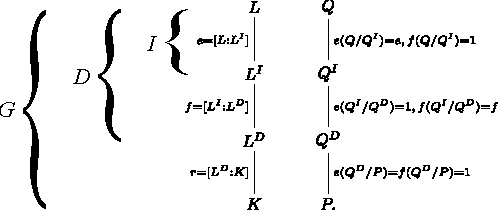
\includegraphics{resources/marcus-inertia-decomp}
\end{center}
\end{thm}

\begin{rem}
Given $L/K$, we may figuratively say that all ramification of $P$ occurs
between $L^I \subset L$, all residual extension at $P$ occurs between $L^D
\subset L^I$, and all ``topological covering near $P$'' occurs between $K
\subset L^D$ (or perhaps we might say that $$\Spec{\O_{L^D}} \rightarrow
\Spec{\OK}$$ is a regular covering space in a sufficiently small neighborhood
of $P\in \Spec{\OK}$).
\end{rem}

\begin{rem}
The fields $L^I, L^D$ are called the ``inertia field'' and ``decomposition
field,'' respectively.
\end{rem}

It follows from the above theorem (see \cite[Cor.~1,p.~101]{M}) that the
homomorphism from the decomposition group to the residual Galois group is
surjective with kernel $I$ so that we have the exact sequence \[\xymatrix{
1\ar[r] & I(Q/P) \ar[r] & D(Q/P) \ar[r] & \Gal{k(Q)/k(P)} \ar[r] & 1.}\]
Recall that the the extension of finite fields $k(Q)/k(P)$ has degree $f$ so
that its Galois group is cyclic of order $f$.

\begin{cor}
If $D$ is a normal subgroup of $G$ then $P$ splits into $r$ distinct primes in
$L^D$. If, moreover, $I$ is normal in $G$, then each of them remains prime (is
``inert'') in $L^I$. Each one becomes an $e$th power in $L$.
\end{cor}
\begin{proof} \cite[Cor.~2, p.~102]{M}.
\end{proof}

Put $\omega := e^{2\pi i/m}$ and fix a prime $p\in\Z$. Then we have (see
\cite[p.~75]{M}) \[p.\Z[\omega] = (Q_1\cdots Q_r)^{e}\] with the $Q_i$ distinct
primes of $\Z[\omega]$, all of which have the same residual degree $f$ over
$p$. We also have $efr = \varphi(m).$ Moreover, a theorem from \cite[p.~76]{M}
tells us that if we write $m=p^k n$ with $p\ndiv n$, then we have
$e=\varphi(p^k)$ and $f$ is the order of $p$ in the group $(\Z/n)^\times$.

Now let us consider how the theory above applies to the splitting of the prime
$2$ in the field $\Q[\omega_{23}]$ where $\omega_{23} := e^{2\pi i/23}.$

We know that 2 splits into two primes in $\Q[\omega_{23}]$ since $efr = 22$
(because 23 is prime), and $e=1,f=11$. Thus the decomposition field
$\Q[\omega_{23}]^D$ has degree 2 over \Q{}. Moreover, there is exactly one
quadratic subfield of $\Q[\omega_{23}]$ since the Galois group is cyclic of
order 22. Thus the decomposition field must be $\Q[\sqrt{-23}]$ (since by
\cite[Ch.~2, Ex.~8]{M}, $\Q[\sqrt{-23}] \subset \Q[\omega_{23}]$ --- the
exercise says that if $p$ is an odd prime then $\Q[e^{2\pi i/p}]$ contains
$\sqrt{p}$ if $p \equiv 1 \imod{4}$ and $\sqrt{-p}$ if $p\equiv -1 \imod{4}$).
Since 2 is unramified in $\Q[\omega_{23}]$ the inertia field is all of
$\Q[\omega_{23}]$.

In the same vein, if $L/K$ is Galois with cyclic Galois group and $P$ is a
prime in $K$ which splits into $r$ primes in $L$ then the decomposition field
is the unique intermediate field of degree $r$ over $K$ and $P$ splits into $r$
primes in every intermediate field containing the decomposition field.

Let us state without proof the following result (\cite[Theorem 29,p.~104]{M}).

\begin{thm}
With the notations above, among field extensions $K'$ intermediate to $L/K$, we
have that

(1) $L^D$ is maximal such that there is a prime $P'/P$ such that $$e(P'/P) =
f(P'/P) = 1,$$

(2) $L^D$ is minimal such that $Q$ is the only prime of $L$ lying over some
prime $P'$,

(3) $L^I$ is maximal such that $e(P'/P)=1$; thus it is also known as the
maximal unramified subextension of $L/K$, and

(4) $L^I$ is minimal such that $Q$ is totally ramified over $P'$ (i.e.~such
that $e(Q/P') = [L:K']).$
\end{thm}

We turn our attention next to quadratic reciprocity.

%%%%%%%%%%%%%%%%%%%%%%%%%%%%%%%%%%%%%%%%%%%%%%%%%%%%%%%%%%%%%%%%%%%%%%

\section{Quadratic Reciprocity}

\renewcommand{\O}{\ensuremath{\mathcal{O}}}

\begin{defn}
A prime $P$ of a number field $K$ is said to split completely in a extension
field $F$ if $P$ splits into $[F:K]$ distinct primes, so that all must have
$e=f=1$.
\end{defn}

Conversely, if all primes of $F$ above $P$ have $e=f=1$ then $P$ must split
completely in $F$. (All of these statements follow from the $n=efr$ theorem.)
Thus if a prime splits completely in some extension, then it splits completely
in every intermediate extension.

The results from the last lecture easily imply (in our usual notational setup)
the following

\begin{cor}\label{split}
If $D := D(Q/P)$ is a normal subgroup of $G := \Gal{L/K}$ then $P$ splits
completely in $K'$ iff $K' \subset L^D$.
\end{cor}

For the proof, see \cite[p.~105]{M}. We will be interested in applying this in
the case where $G$ is abelian so that all subgroups are automatically normal.

\begin{defn}
Let $p\in \Z$ be an odd prime. For $n\in\Z$ prime to $p$, we define the
Legendre symbol by
\[\left( \frac{n}{p} \right) :=
\begin{cases}
  1 & \text{if } n \text{ is a square mod } p, \\
  -1 & \text{otherwise.}
\end{cases} \]
\end{defn}


\begin{thm}[Quadratic Reciprocity] We have
    \[
    \left( \frac{2}{p} \right) =
    \begin{cases}
        1 & \text{if } p \equiv \pm 1 \imod{8}, \\
        -1 & \text{if } p \equiv \pm 3 \imod{8} \\
    \end{cases}
    \] and for odd primes $q\neq p$ we have
    \[
    \left( \frac{q}{p} \right) =
    \begin{cases}
        \left( \frac{p}{q} \right) & \text{if } p \text{ or } q \equiv 1 \imod{4}, \\
        -\left( \frac{p}{q} \right) & \text{if } p \equiv q \equiv 3 \imod{4}.
    \end{cases}
    \]
\end{thm}

Let us establish a criterion for a prime to be a $d$th power mod $p$, for any
$d|p-1$. Put $\omega := \omega_p := e^{2\pi i/p}$ and consider $\Q[\omega].$
Since $\Gal{\Q[\omega]/\Q} \simeq \Z/(p-1)$, there exists for each $d|p-1$ a
unique subfield $F_d \subset \Q[\omega]$ of degree $d$ over \Q{}, and $F_d
\subset F_{d'}$ iff $d|d'$.

\begin{thm}\label{fdsplit}
Let $p$ be an odd prime and $q\neq p$ be any other prime. Let $d| p-1$. Then
$q$ is a $d$th power mod $p$ iff $q$ splits completely in $F_d$.
\end{thm}

\begin{proof}
We know\footnote{This result was reviewed in the previous lecture in the course
of working out the example on the splitting of 2 in $\Q[\omega_{23}].$} that
$q$ splits into $r$ distinct primes in $\Q[\omega]$, where $f := (p-1)/r$ is
the order of $q$ in $(\Z/p)^\times$. This group is cyclic of order $p-1$ so
the map $x \mapsto x^d$ is a group homomorphism whose image is the unique
subgroup of order $(p-1)/d$; it consists of all the elements of
$(\Z/p)^\times$ whose orders divide $(p-1)/d$. Thus the following are
equivalent

(i) $q$ is a $d$th power mod $p$

(ii) $f|(p-1)/d$

(iii) $d|r$

(iv) $F_d \subset F_r$

Now, the decomposition field of a prime $Q$ of $\Q[\omega]$ lying over $q\in
\Z$ must have degree $r$, and therefore this decomposition field must be $F_r$
since that is the only intermediate field of degree $r$.

Therefore the condition $F_d \subset F_r$ is equivalent to the condition that
$q$ splits completely in $F_d$, by Corollary \ref{split}, and the theorem is
proved.
\end{proof}

\begin{lem}
If $p$ is an odd prime then $\Q[e^{2\pi i/p}]$ contains $\sqrt{p}$ if $p \equiv
1 \imod{4}$ and $\sqrt{-p}$ if $p\equiv -1 \imod{4}$
\end{lem}
\begin{proof} This is exercise 8 of chapter 2 of \cite{M}.
\end{proof}

\begin{proof}[Proof of Quadratic Reciprocity]
We have \[\left( \frac{q}{p} \right) = 1\] iff $q$ splits completely in $F_2$
iff $F_2 \subset F_r$ where $r:= $ the number of distinct primes that $q$
splits into in $\Q[\omega_p]$, and where $\omega_p := e^{2\pi i /p}$. Now
$F_2$ is the unique quadratic extension of \Q{} intermediate to
$\Q[\omega_p]/\Q$. By the above lemma, we see that
\[ F_2 =
\begin{cases}
  \Q[\sqrt{p}] & \text{if } p \equiv 1 \imod{4},\\
  \Q[\sqrt{-p}] & \text{if } p \equiv -1 \imod{4}.
\end{cases} \] Thus by Theorem \ref{fdsplit} we are reduced to determining how
$q$ factors in $\Q[\sqrt{\pm p}]$. This is accomplished by the following
Proposition. In greater detail, we argue as follows.

Let us compute $(\frac{2}{p})$. We perform a case analysis on $p\imod{8}.$

$p\equiv 1 \imod{8} \Rightarrow p \equiv 1 \imod{4} \Rightarrow \Q[\sqrt{p}]
\subset \Q[\omega_p]$. Then, in the notation of the next proposition, we have
$m = p \equiv 1 \imod{4}$ so that $2$ is split by $(*)$. Therefore
$(\frac{2}{p}) = 1$.

$p\equiv 7 \imod{8} \Rightarrow p \equiv -1 \imod{4} \Rightarrow \Q[\sqrt{-p}]
\subset \Q[\omega_p] \Rightarrow m = -p \equiv -7 \imod{8} \Rightarrow m \equiv
1 \imod{8} \Rightarrow 2$ is split by $(*)$ and therefore $(\frac{2}{p}) = 1$.

$p\equiv 3 \imod{8} \Rightarrow p \equiv -1 \imod{4} \Rightarrow \Q[\sqrt{-p}]
\subset \Q[\omega_p] \Rightarrow m = -p \equiv -3 \equiv 5 \imod{8} \Rightarrow
2$ is inert and therefore $(\frac{2}{p}) = -1$.

$p\equiv 5 \imod{8} \Rightarrow p \equiv 1 \imod{4} \Rightarrow \Q[\sqrt{p}]
\subset \Q[\omega_p] \Rightarrow m = p \equiv 5 \imod{8} \Rightarrow 2$ is
inert and therefore $(\frac{2}{p}) = -1$.

Let us now compute $(\frac{q}{p})$ for $p,q$ distinct odd primes.

We have:

$p\equiv 1 \imod{4}$ and $(\frac{q}{p}) = 1 \Leftrightarrow q.\O$ splits
completely in $\Q[\sqrt{p}] \Leftrightarrow m = p $ and $p \equiv a^2 \imod{q}$
for some $a$ $\Leftrightarrow (\frac{p}{q}) = 1$.

$p\equiv 3 \imod{4}$ and $(\frac{q}{p}) = 1 \Leftrightarrow q.\O$ splits
completely in $\Q[\sqrt{-p}] \Leftrightarrow m = -p $ and $-p \equiv a^2
\imod{q}$ for some $a$ $\Leftrightarrow 1 = (\frac{q}{p}) = (\frac{-p}{q}) =
(-1)^{\frac{q-1}{2}}(\frac{p}{q})$. Thus in this case we have:

(case $(\frac{p}{q}) = 1$): $1 = (\frac{q}{p}) = (-1)^{\frac{q-1}{2}}
\Leftrightarrow q \equiv 1 \imod{4}$ (i.e. $p$ or $q\equiv 1 \imod{4}$)

and

(case $(\frac{p}{q}) = -1$): $1 = (\frac{q}{p}) = -(-1)^{\frac{q-1}{2}}
\Leftrightarrow q \equiv 3 \imod{4}$ (i.e. $p\equiv q\equiv 3 \imod{4}$).
\end{proof}

\begin{rems}
(a) We may give a concise statement of quadratic reciprocity, valid in all
cases: \[\left( \frac{q}{p} \right) = (-1)^{\frac{p-1}{2}\frac{q-1}{2}} \left(
\frac{p}{q} \right).\]

(b) In the above proof, we used the fact that the quadratic symbol may
alternatively be defined by \[\left( \frac{a}{p} \right) := a^{\frac{p-1}{2}}
\imod{p}\] which makes it clear that it is gives rise to a homomorphism
$(\Z/p)^\times \rightarrow \{\pm 1\}$. [see, for instance, the Wikipedia page
on the Legendre symbol.]
\end{rems}

\begin{prop}
Let $\ell\in \Z$ be a prime and let \O{} be the ring of integers in the
quadratic field $\Q[\sqrt{m}]$ where $m$ is squarefree. Recall that $\O$ has
integral basis $\{1,\sqrt{m}\}$ and discriminant $4m$ when $m\equiv
2,-1\imod{4}$ and integral basis $\{1,(1+\sqrt{m})/2\}$ and discriminant $m$
when $m\equiv 1\imod{4}.$

We have

(i) if $\ell|m$ then $\ell.\O = (\ell,\sqrt{m})^2$,

(ii) if $m$ is odd then \[2.\O =
\begin{cases}
    (2,1+\sqrt{m})^2 & \text{if } m\equiv -1 \imod{4},\\
    (2,(1+\sqrt{m})/2)(2,(1-\sqrt{m})/2 & \text{if } m\equiv 1 \imod{8},
    \;\;\;\;\;\;\;\; \;\;\;\;\;\;\;\; (*) \\
    \text{prime if } m\equiv 5 \imod{8}.
\end{cases} \]

(iii) if $\ell$ is odd and $\ell\ndiv m$ then \[\ell.\O =
\begin{cases}
    (\ell,n+\sqrt{m})(\ell,n-\sqrt{m}) & \text{if } m \equiv n^2
    \imod{p}, \;\;\;\;\;\;\;\; \;\; (**)\\
    \text{prime if } m \text{ is not a square mod } p.
\end{cases} \] and in cases $(*)$ and $(**)$, the factors are
distinct.
\end{prop}
\begin{proof} See \cite[25, p.~74]{M}.
\end{proof}

\bigskip

We now turn our attention to the Frobenius automorphism.

\bigskip

\begin{defn}
Assume that the prime $P$ of $K$ is unramified in $L$, so that $I(Q/P)$ is
trivial. Then we have an isomorphism \[D(Q/P) \xrightarrow{\sim}
\Gal{k(Q)/k(P)}.\] The latter Galois group has the distinguished generator
\[\overline{x}\mapsto \overline{x}^{\norm{P}}\] and the corresponding
automorphism $\varphi\in D$ has the property that \[\varphi(x) \equiv
x^{\norm{P}} \imod{Q}\] for all $x\in \OL{}$. Moreover, $\varphi$ is uniquely
determined in $D$ and hence in $G$. We denote this automorphism by
\[\Fr{Q/P}.\] It is known as the \textit{Frobenius automorphism} of $Q/P$. One
directly verifies that $$\Fr{\sigma Q/P} = \sigma \Fr{Q/P} \sigma^{-1}$$ for
$\sigma\in G$ so that the conjugacy class of \Fr{Q/P} depends only on $P$, thus
if $G = \Gal{L/K}$ is abelian, the Frobenius automorphism depends only on $P$
and we may write \(\Fr{P}\) for the element of $G$ such that \[\Fr{P}(x) \equiv
x^{\norm{P}} \imod{P.\OL}.\]
\end{defn}

\bigskip

Let us see what all this means for the cyclotomic fields. Put $L :=
\Q[\omega],\omega := e^{2\pi i/m}$ and $K:= \Q$. Then $G \simeq (\Z/m)^\times$
with $\sigma\in G$ corresponding to $k\in (\Z/m)^\times$ iff $\sigma(\omega) =
\omega^k$. We may consider \Fr{p} for all unramified primes, i.e.~for all
primes $p\ndiv m$ (this is explicitly proved in Washington, Introduction to
Cyclotomic Fields, page 10). We have \[\Fr{p}(x) \equiv x^p \imod{
p.\Z[\omega]}\] for all $x\in \Z[\omega].$ Since the automorphism $\sigma_p :
\omega \mapsto \omega^p\in G$ satisfies this congruence, and since $G$ is
abelian so that the Frobenius automorphism is uniquely determined as an element
of $G$, we must have that $\sigma_p : \omega\mapsto\omega^p \in G$ coincides
with \Fr{p}. For an arbitrary element $x = \sum a_i \omega^i \in \Z[\omega]$
we have \[\sigma_p\left( \sum a_i \omega^i \right) = \sum a_i \omega^{pi}\] and
thus \[\sum a_i \omega^i \equiv \left( \sum a_i \omega^i \right)^p
\imod{p.\Z[\omega]}.\]

\begin{rem}
It follows from the results proved in chapter 4 that $p$ is ramified in an
extension of \Q{} iff $p$ divides the discriminant. See \cite[Theorem 34,
p.~112]{M}.
\end{rem}

%%%%%%%%%%%%%%%%%%%%%%%%%%%%%%%%%%%%%%%%%%%%%%%%%%%%%%%%%%%%%%%%%%%%%%
\bibliography{bib}
\end{document}
